
% TODO: intro. to core(s) the ISEs are integrated with

The ISE designs were integrated with the \CORE{2} core as a base platform
for evaluation.
The \CORE{2}\footnote{%
  \ifbool{anonymous}{Details of this core have been anonymised to comply with the TCHES submission guidelines.}{}
} core
implements the {\tt rv32imc} instruction set: 32-bit base ISA, with the
Multiply and Compressed instruction set extensions.
A block diagram of the core is shown in~\REFFIG{fig:design:cpu_block:2}.
A standard 5-stage, in-order pipeline is used, which
means that each stage of execution
(namely fetch, decode, execute, memory access, and write-back)
occurs in {\em parallel} for multiple different in-flight instructions.

Note there are two memory interfaces, one for (instruction) fetch and one for
(data) memory accesses;
no form of cache hierarchy or branch prediction is implemented.
The core implements various performance counters,
and
elements of the
RISC-V Privileged Resource Architecture (PRA)~\cite[Chapter 3]{RV:ISA:II:17}
related to exception and interrupt handling.

\begin{figure}
\centering
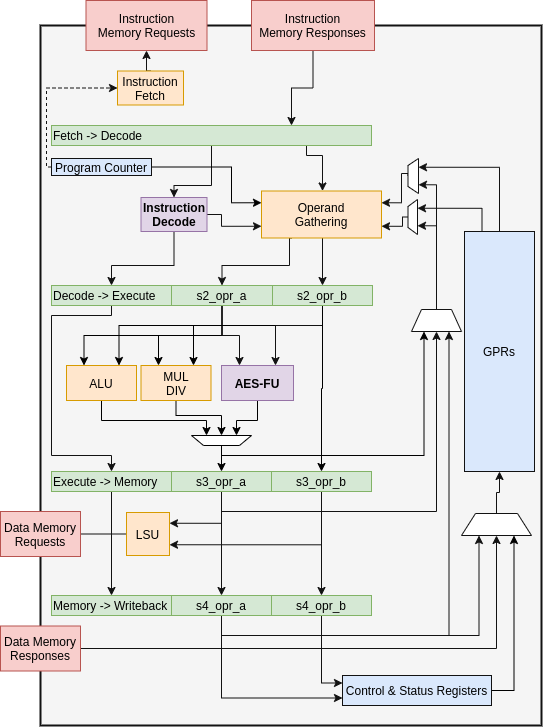
\includegraphics[scale=0.5,angle=90]{diagrams/scarv-cpu-uarch.png}
\subcaption{Core $2$: \CORE{2}.}
\label{fig:design:cpu_block:2}
\end{figure}
